\documentclass[border=15pt, multi, tikz]{standalone}
\usepackage{import}
%%
% Using PlotNerualNet: https://doi.org/10.5281/zenodo.2526396
% To generate: pdflatex <filename>
%%
\subimport{/Users/theeel/src/laTex/PlotNeuralNet/layers/}{init}
\usetikzlibrary{positioning}
\usetikzlibrary{3d} %for including external image 

\def\InputColor{rgb:red,5;green,5;blue,5;white,5}
\def\ConvColor{rgb:yellow,5;red,2.5;white,5}
\def\InvResColor{rgb:yellow,0;red,5;white,5}
\def\ConvReluColor{rgb:yellow,5;red,5;white,5}
\def\PoolColor{rgb:red,1;black,0.3}
\def\DcnvColor{rgb:blue,5;green,2.5;white,5}
\def\SoftmaxColor{rgb:magenta,5;black,7}
\def\SumColor{rgb:blue,5;green,15}

\begin{document}
\begin{tikzpicture}%[x=1cm, y=1cm, z=1cm]
\tikzstyle{connection}=[ultra thick,every node/.style={sloped,allow upside down},draw=\edgecolor,opacity=0.7]
%%%%%%%%%%%%%%%%%%%%%%%%%%%%%%%%%%%%%%%%%%%%%%%%%%%%%%%%%%%%%%%%%%%%%%%%%%%%%%%%%%%%%%%%
%% Draw Layer Blocks
%%%%%%%%%%%%%%%%%%%%%%%%%%%%%%%%%%%%%%%%%%%%%%%%%%%%%%%%%%%%%%%%%%%%%%%%%%%%%%%%%%%%%%%%

% The input image
% The input layer
% There is a 5x multiplyer: 0.2* 213.3 = 42.66
%\begin{scope}[shift={(0,-10,0)}] % shift everything down in 3D
\node[canvas is zy plane at x=0] (temp) at (-1,-5,0) {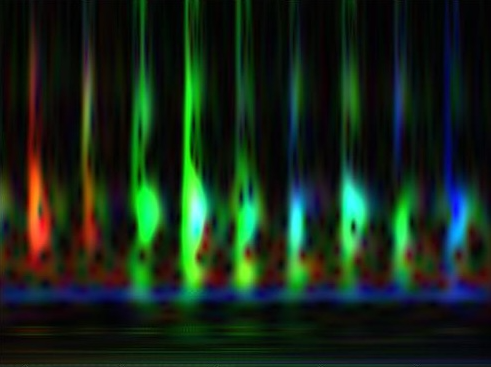
\includegraphics[width=42.66 cm,height=5.18 cm]{cwt.png}};

\pic[shift={(2,-5,0)}] at (0,0,0) 
        {Box={name=input,caption=Input,%
              xlabel={{"9x256","dummy"}},zlabel="    2133",
              fill=\InputColor,%
              height=25.9,width=0.9,depth=213.3}
         };

%%
% Output Shapes: note: in cm
%%


% Convolve2D, Group Norm, RFeLU6
\pic[shift={(4,0,0)}] at (input-east)
    {RightBandedBox={ name=inpConv, caption=Conv, xlabel={{"32x128", }}, zlabel=1067,
        fill=\ConvColor,bandfill=\ConvReluColor,%
        height=12.8,width=3.2,depth=107 } };

% Inverted Res 1
\pic[shift={(2,0,0)}] at (inpConv-east) {RightBandedBox={name=invRes1,caption=InvRes,%
        xlabel={{"16x128", }},zlabel=1067,fill=\InvResColor,bandfill=\ConvReluColor,%
        height=12.8,width=1.6,depth=106.7}};
% Inverted Res 2, 3
\pic[shift={(2,0,0)}] at (invRes1-east) {RightBandedBox={name=invRes2,caption=InvRes,%
        xlabel={{"24x64",}},zlabel=534,fill=\InvResColor,bandfill=\ConvReluColor,%
        height=6.4,width={2.4,2.4},depth=53.4}};
% Inverted Res 4, 5, 6
\pic[shift={(1.8,0,0)}] at (invRes2-east) {RightBandedBox={name=invRes4,caption=InvRes,%
        xlabel={{, "32x32", }},zlabel=267,
        fill=\InvResColor,bandfill=\ConvReluColor,%
        height=3.2,width={3.2, 3.2, 3.2},depth=26.7}};
% Inverted Res 7, 8, 9, 10
\pic[shift={(1.5,0,0)}] at (invRes4-east) {RightBandedBox={name=invRes7,caption=InvRes,%
        xlabel={{,"64x16", ,}},zlabel=134,fill=\InvResColor,bandfill=\ConvReluColor,%
        height=1.6,width={6.4,6.4,6.4,6.4},depth=13.4}};
% Inverted Res 11, 12, 13
\pic[shift={(1.5,0,0)}] at (invRes7-east) {RightBandedBox={name=invRes11,caption=InvRes,%
        xlabel={{,"96x16", }},zlabel=134,fill=\InvResColor,bandfill=\ConvReluColor,%
        height=1.6,width={9.6,9.6,9.6},depth=13.4}};
% Inverted Res 14, 15, 16
\pic[shift={(1.5,0,0)}] at (invRes11-east) {RightBandedBox={name=invRes14,caption=InvRes,%
        xlabel={{,"160x8", ,}},zlabel=67,fill=\InvResColor,bandfill=\ConvReluColor,%
        height=0.8,width={16,16,16},depth=6.7}};
% Inverted Res 17
\pic[shift={(1.5,0,0)}] at (invRes14-east) {RightBandedBox={name=invRes17,caption=InvRes,%
        xlabel={{"320x8",}},zlabel=67,fill=\InvResColor,bandfill=\ConvReluColor,%
        height=0.8,width={32},depth=6.7}};

% Conv2d, NormActivation
\pic[shift={(1.5,0,0)}] at (invRes17-east) {RightBandedBox={name=conv18,caption=Conv-GroupNorm-ReLU,%
        xlabel={{"1280x8",}},zlabel=67,fill=\ConvColor,bandfill=\ConvReluColor,%
        height=0.8,width={128},depth=6.7}};

%%%%%%%%%%%%%%%%%%%%%%%%%%%%%%%%%%%%%%%%%%%%%%%%%%%%%%%%%%%%%%%%%%%%%%%%%%%%%%%%%%%%%%%%%    
%%% Output
%%%%%%%%%%   
%AdaptiveAvgPool2d
\pic[shift={(0,0,0)}] at (conv18-east) {Box={name=pool1,caption=AdaptiveAvePool,%
        fill=\PoolColor,opacity=0.5,height=0.8,width=128,depth=6.7}};

%self.fc = nn.Linear(lastLayerFeatureMap_size, numOutputs)
\pic[shift={(1,0,0)}] at (pool1-east) {Box={name=fc,caption=fc,%
        xlabel={{1,}},fill=\ConvColor,%
        height=1,width=1,depth=1,zlabel=}};


%%%%%%%%%%%%%%%%%%%%%%%%%%%%%%%%%%%%%%%%%%%%%%%%%%%%%%%%%%%%%%%%%%%%%%%%%%%%%%%%%%%%%%%%
%% Draw connections
%%%%%%%%%%%%%%%%%%%%%%%%%%%%%%%%%%%%%%%%%%%%%%%%%%%%%%%%%%%%%%%%%%%%%%%%%%%%%%%%%%%%%%%%
\draw [connection]  (input-east)    -- node {\midarrow} (inpConv-west);
\draw [connection]  (inpConv-east)    -- node {\midarrow} (invRes1-west);
\draw [connection]  (invRes1-east)    -- node {\midarrow} (invRes2-west);
\draw [connection]  (invRes2-east)    -- node {\midarrow} (invRes4-west);
\draw [connection]  (invRes4-east)    -- node {\midarrow} (invRes7-west);
\draw [connection]  (invRes7-east)    -- node {\midarrow} (invRes11-west);
\draw [connection]  (invRes11-east)    -- node {\midarrow} (invRes14-west);
\draw [connection]  (invRes14-east)    -- node {\midarrow} (invRes17-west);
\draw [connection]  (invRes17-east)    -- node {\midarrow} (conv18-west);
\draw [connection]  (pool1-east)    -- node {\midarrow} (fc-west);
%%%%%%%%%%%%%%%%%%%%%%%%%%%%%%%%%%%%%%%%%%%%%%%%%%%%%%%%%%%%%%%%%%%%%%%%%%%%%%%%%%%%%%%%

%\end{scope}  % End shift
\end{tikzpicture}
\end{document}\grid

